\chapter{Introduction}
Which proteins are involved in chemical synapses? How do proteins interact? These questions and many more arise in biology and related sciences. Microscopy is a powerful tool to answer these questions, because it gives information about the shape and position of components of cells, the distribution of proteins and more. However light microscopy is limited in spatial resolution due to limited diffraction, as described by \cite{Abbe} \footnote{There is a fundamental limit for the resolution of optical systems. It is roughly half the wavelength of the light which is used for microscopy. With green light of 500 nm this means the minimal resolution achievable is about 250 nm}. Recently there have been developed different methodes to increase the resolution of light microscopy beyond the diffraction limit. To name a few: Photoactivated Localization Microscopy (PALM) (\cite{Palm}), Stochastic Optical Reconstruction Microscopy (STORM) (\cite{Storm}) or Stimulated Emission Depletion STED (\cite{sted}).\newline
For these techniques many images with sparsely distributed signals, coming from fluorophors, that are attached to the sample are used. Special fluorophores are used that activate only with a low probability, which means that there are less fluorophores activated at a certain time. The the pointlike fluorophores are blured by diffraction. Because the signals are sparse the center of each signal can be determined with sub pixel accuracy. This is not possible for one image with all signals, where the blurred point spread functions overlap and are undistinguishable. There are different ways to stain the biological sample with fluorophors. One way is to use antibodies which bind to specific targets within a cell. The antibody is either directly linked to a fluorophore or two antibodies are used, where the first binds to the biological structre and the second with the fluorophore attached to the first antibody. 
\newline
For this thesis only the STORM method is considered. It can be used to investigate the distribution of different proteins within a cell for example. To do so each kind of protein is labeled with a certain fluorophore. The images shown in this thesis were aquired to show signals from only one kind of fluorophore per channel. However, to be able to seperate the different signals from the fluorophores, their emission spectrum must be distinct. This leads to cromatic aberration which results in images that are distorted and thus can not be aligned easily.\newline 
Many research groups have developed their own software to process STORM data sets. But most of these programs need many parameters, like a threshold for background suppression or the camera parameters, that must be set by the user to get reasonable results. Therefore these programs are difficult to use for somebody who is not familiar with image processing or does not know the parameters influence on the results.\newline

One key question of this thesis is how to build software that is easy to use even without prior information about the data or knowledge of image processing? \newline

Our answer to this question is SimpleStorm. A software that calibrates itself. It estimates the camera parameters and the width of the point spread function of the fluorophores. In contrast to many other software applications, no threshold is needed. To provide this feature a robust background estimation was applied.\newline

If more than one kind of fluorophore was used to stain the sample, the resulting images are distorted relative to each other due to chromatic aberration. The Colorcomposer tool was developed to do align multiple images automatically and to analyse the aligned images. Figure \ref{dualcolor} shows both an reconstructed and aligned STORM image in the upper part and the maximum projection over all frames of the raw data in the lower part. The colocalization of the molecules of the different channels is a useful measure in biology to determine whether or not near molecules might interact. The Colorcomposer software calculates both global and local measures of localization.

\begin{figure}
\centering
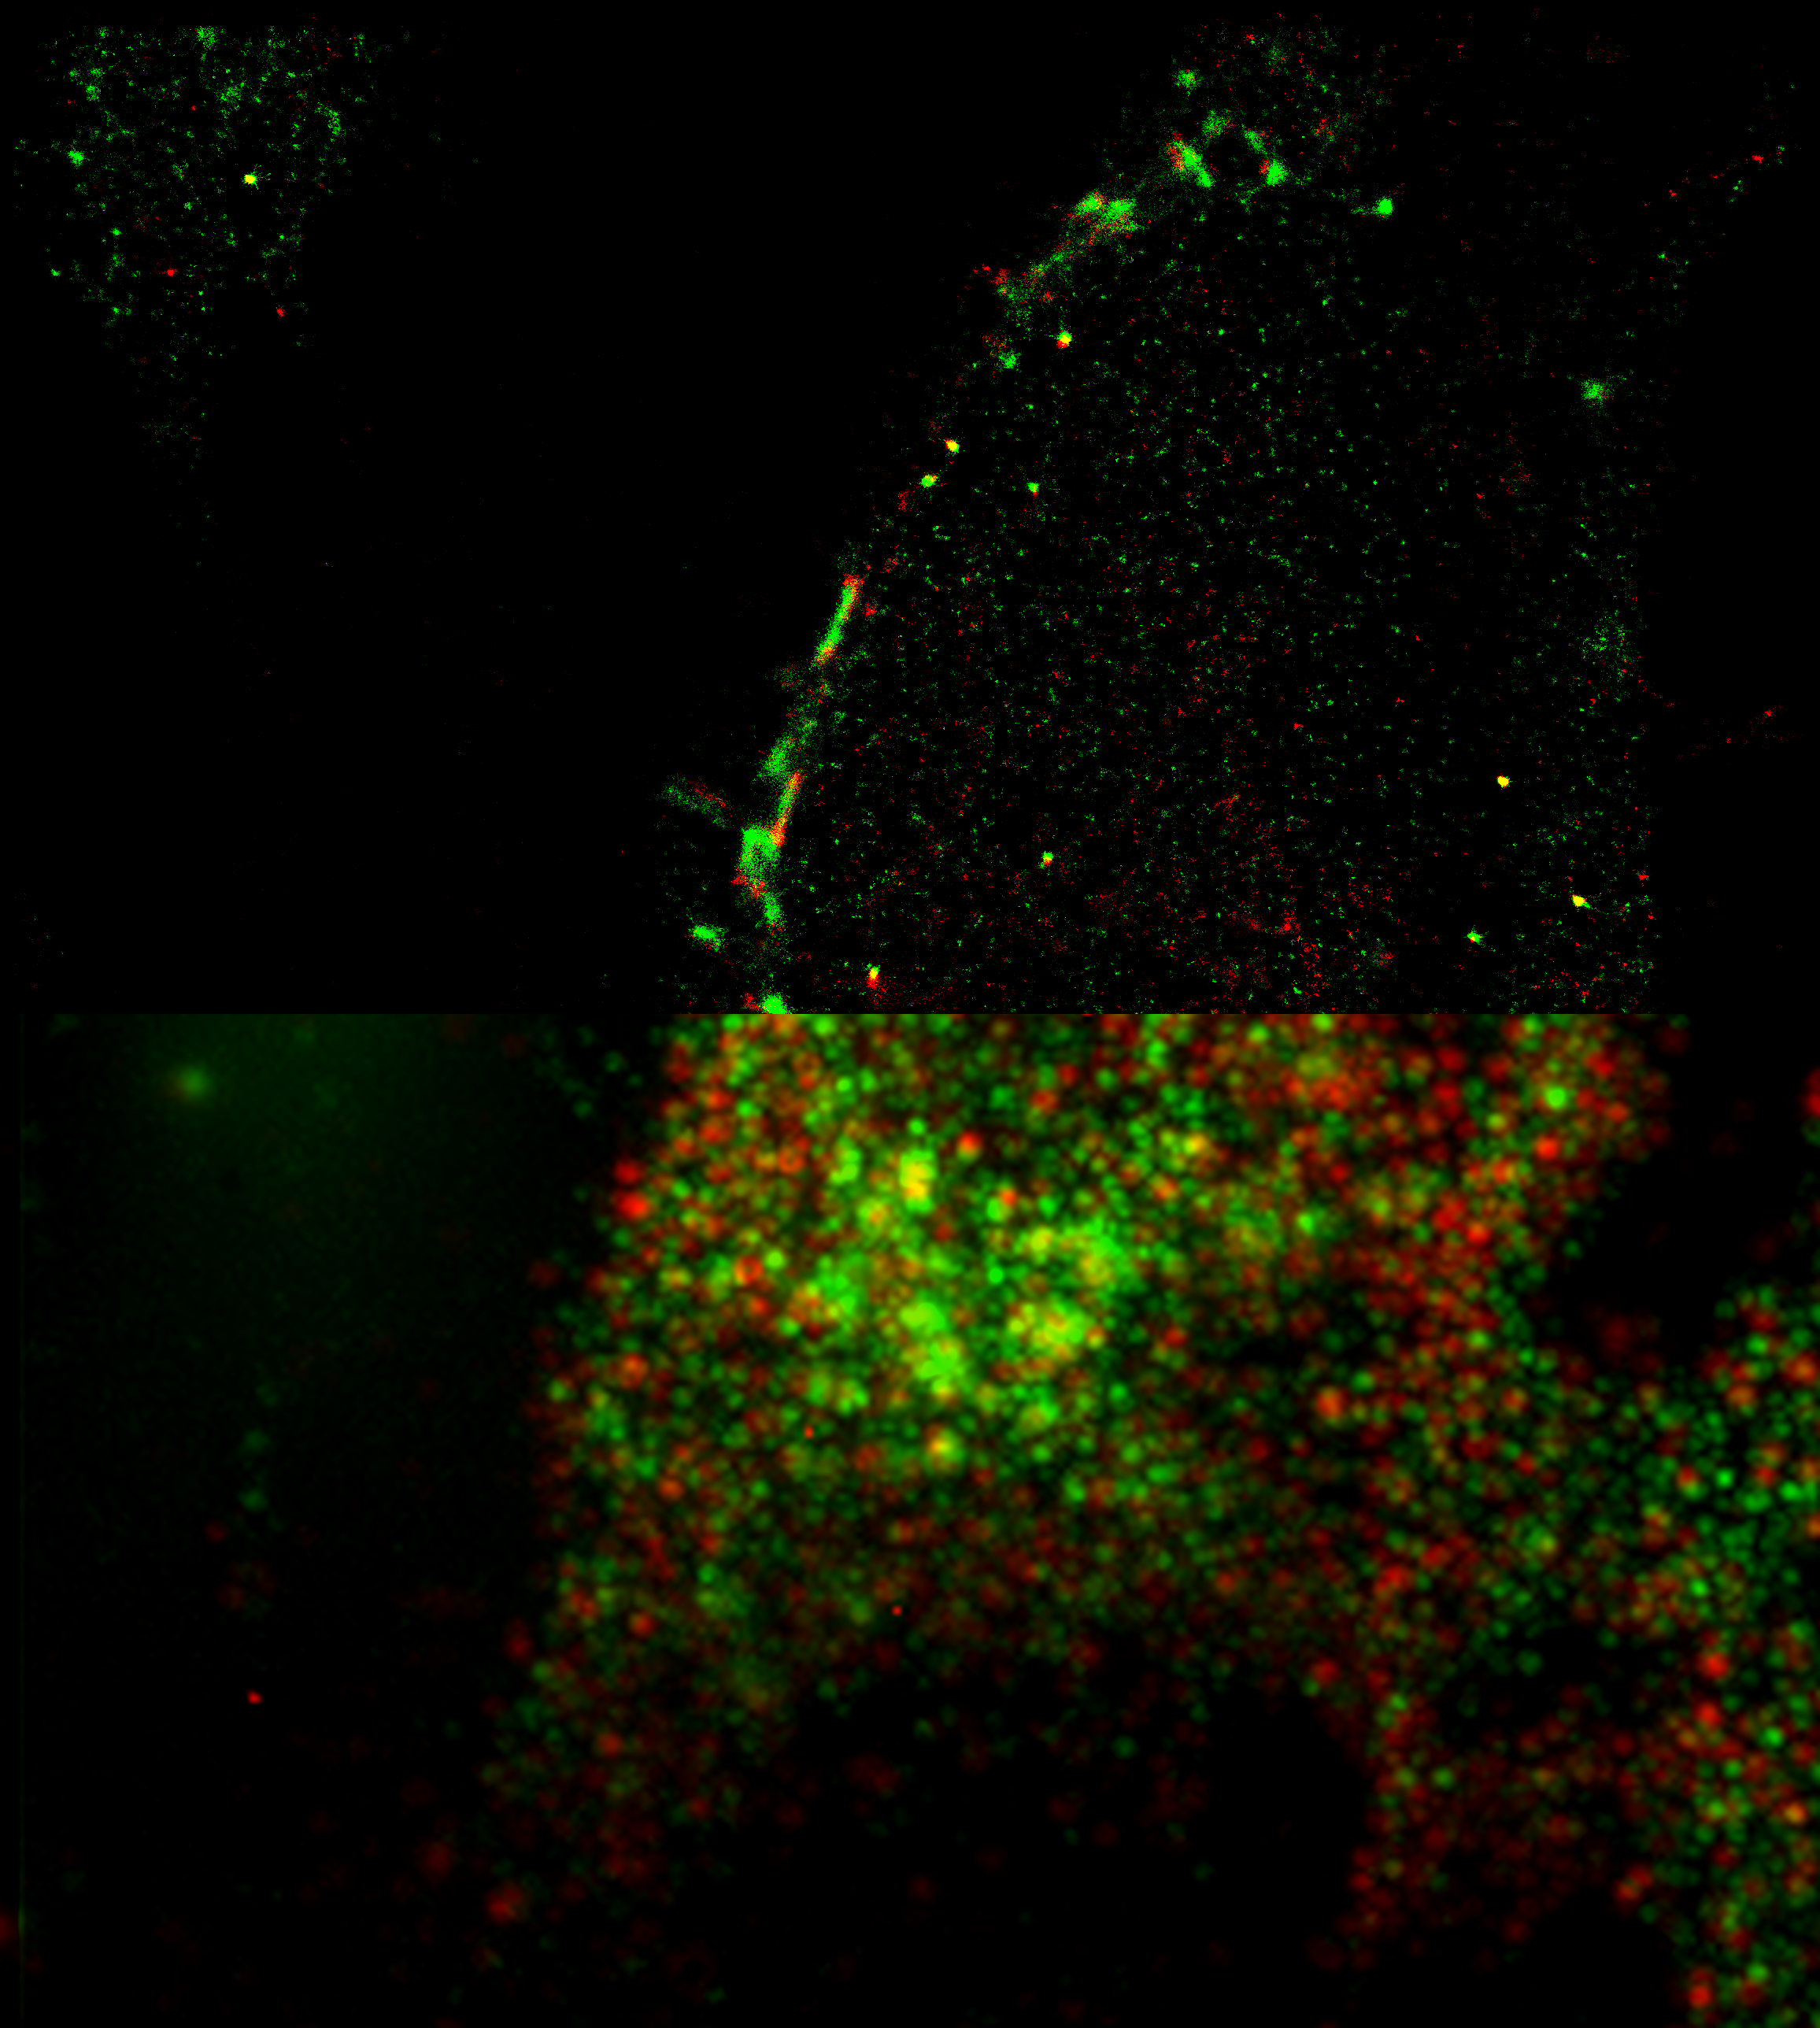
\includegraphics[width = 0.88\textwidth]{pictures/alignedStormWidefield.png}
	\caption{Dual-color image of a cell treated with nocodazole. The upper part shows the reconstructed and aligned image, the lower part the maximum projection of the raw data over all frames.}
	\label{dualcolor}
\end{figure}


